\documentclass{article}

\usepackage[utf8]{inputenc}
\usepackage{mathtools}

\title{Simulação de Redes 5G no NS-3}
\author{Renê Cardozo}
\date{}

\begin{document}
\maketitle
\section{Módulos}
Oficialmente existem dois módulos na NS-3 App Store: 5G-LENA e mmWave Cellular Network Simulator. [1][2]

\section{mmWave}
Produzido em Novembro de 2015, o artigo "5G MmWave Module for the ns-3 Network Simulator" [3] apresenta o módulo mmWave para o ns-3.

\subsection{Resumo do Artigo}
O simulador de redes ns-3 já possui uma ampla gama de protocolos implementados, sendo uma importante ferramenta pra o estudo e design de protocolos e suas interações entre diferentes camadas. Já são implementados no simulador módulos para WiFi, WiMAX e 3GPP-LTE. mmWave foi o primeiro módulo proposto para a simulação baseada em ondas milimétricas.

O módulo é inspirado em outro já disponível para a simulação de redes LTE/EPC (Long Term Evolution/Evolved Packet Core), chamado LENA. No mmWave são implementadas as camadas PHY (física) e MAC (parte da camada de enlace de dados).

Com o objetivo de reduzir a latência, sistemas 5G implementam a estrutura 'Time Division Duplex' (TDD), na qual cada frame é dividido em um número de subframes de tamanho pré-fixado pelo usuário. Cada subframe, por sua vez, é dividido em um número de slots com duração fixa. Cada slot possui um número específico de símbolos OFDM (Orthogonal Frequency-Division Multiplexeing). Cada um destes slots pode ser de controle ou dados, e são dedicados para uplink (UL) ou downlink (DL). 

A estrutura dos frames pode ser totalmente customizada pelo usuário através do objeto mmwavePhyMacCommon que armazena todos os valores especificados pelo usuário para os parâmetros utilizados pelo simulador.

\begin{figure}[!h]
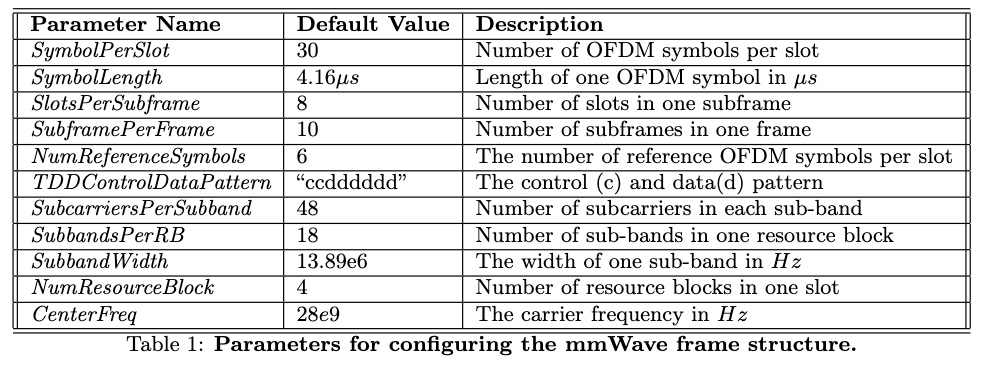
\includegraphics[width=\textwidth]{tabela-parametros-frame}
\centering
\end{figure}

** Um simbolo pode ser descrito como um pulso em uma transmissão baseband digital ou um tom em uma transmissão passband. O símbolo pode ser uma forma de onda, um estado ou uma condição do canal de comunicação, que persiste por determinado período de tempo, podendo cada um destes representar um ou mais bits de dados.

\subsubsection{Camada Física}

A camada física é responsável por:
\begin{itemize}
\item Coordenar a transmissão e recepção de sinais.
\item Simular o início e o final de frames, subframes, e slots. (StartTxDataFrames, StartTxControlFrames, StartRx (StartRxData/StartRxControl).
\item Entregar os pacotes de dados e mensagens do controle recebidos do canal para a camada MAC.
\item Modelar o erro de codificação para o sinal recebido e calcula métricas como o SINR (Signal to Interference and Noise Ratio).
\end{itemize}

Utilizando os valores de banda disponível para a transmissão, mmWaveSpectrumValueHelper calcula a densidade energética espectral e usa este valor para a transmissão do sinal. O dispositivo calcula SINR no Indicador de Qualidade do Canal e envia-o a base para alocação de recursos. Sinais de controle são assumidos idealmente transmitidos. 

Também é incorporado um modelo de erros que estipula uma probabilidade com a qual os pacotes devem ser descartados pelo receptor. 

Utilizando os recursos alocados pelo mmWaveEnbMac, o módulo decide a natureza da comunicação de cada slot e a direção da transferência das mensagens (uplink/downlink). No início de cada slot o eNodeB envia uma SubframeIndication para a camada MAC. O subframe de indicação para o primeiro slot inicia as funções de alocação. Os pacotes de dados e mensagens de controle recebidos da camada MAC são armazenados nas filas PacketBurstQueue e ControlMessageQueue, respectivamente, e transmitidos para os dispositivos conectados nos slots alocados.

O cálculo do ganho utilizando múltiplas antenas é crítico para a modelagem de ondas milimétricas. A modelagem deste comportamento é realizada através da classe MultiModelSpectrumChannel, a qual utiliza as classes mmWaveSpectrumPhy(Tx), mmWavePropagationLossModel, mmWaveBeamforming, mmWaveSpectrumPhy(Rx) para obter seus parâmetros. Devido a grande perda de sinal em altas frequências, a geração de feixes de sinal através da utilização de múltiplas antenas é essencial para que os dispositivos sejam atingidos em redes 5g, uma vez que sem esta intensificação de sinal a área coberta por um torre seria muito pequena e insuficiente para atender a demanda.

Para reduzir a complexidade computacional, as matrizes dos canais e os vetores de formação de feixes foram pré-calculados no MATLAB, sendo instanciados ao início da simulação. Uma matrix instanciada é então escolhida randomicamente para cada par dispositivo-eNodeB para caracterizar a ligação, por meio do método m\_channelMatrixMap e das structs BeamFormingParams e ChannelMatrix.

Embora a interferência seja reduzida pela utilização de feixes por meio de várias antenas, a interferência pode ser ainda muito relevante em alguns cenários. Há, portanto, um módulo para o cálculo de interferência baseado no vetor de formação de feixes para cada ligação, buscando calcular o SINR.

\subsubsection{Camada MAC}
A camada MAC é controlada pela classe mmWaveMac, que serve como base para as classes mmWaveEnbMac e mmWaveUeMac, as
quais simulam o comportamento dos eNodebs e dos usuários, respectivamente. O eNodeB está conectado a um agendador, o
qual estipula a alocação de tempo e coordenação de recursos para cada subframe. Todas as frequencias em um slot são
dedicadas a um usuário particular, sendo os slots de controle uma exceção, podendo estes últimos serem usados por
qualquer usuário para transmitir e receber dados da torre.

Os dados são mantidos em filas tanto no eNodeB para cada usuário conectado, como em cada usuário individualmente. O
agendador é responsável por determinar como estes dados serão enviados no subframe indicado para cada transmissão. Sendo
essa decisão notificada para todos os dispositivos da rede pela camada física.

O AMC (Adaptative Modulation and Coding) funciona de maneira similar ao implementado para redes LTE. O usuário mede um
indicador de qualidade do canal (CQI - Channel Quality Indicator), o qual é encaminhado para um eNodeB, sendo provido ao
agendador para computar a melhor modulação e codifiação da conexão. 

O esquema TDD (Time Division Duplex) divide a banda de frequências em subframes, sendo cada qual dividido de acordo com
o tempo ocupado (slot) para uplink e downlink. O modelo permite um melhor aproveitamento da banda, ao contrário do
antigo FDD (Frequency Division Duplex), o qual divide as frequências em espectros dedicados para uplink e downlink. [4] O
módulo divide igualmente os slots temporais entre downlink e uplink.


\section{Referências}
1 - https://apps.nsnam.org/search/?q=5g \\
2 - https://github.com/nyuwireless-unipd/ns3-mmwave \\
3 - https://arxiv.org/abs/1506.08801 \\
4 - https://www.teldat.com/blog/en/tdd-fdd-massive-mimo-for-lte-4g-and-5g/
\end{document}

